%# -*- coding: utf-8 -*-
%%采用 xelatex + ctex 文档类
\documentclass[fancyhdr,fntef,UTF8,oneside,12pt,a4paper, winfonts]{ctexbook}
%%%%%!!!请将您的个人信息按照注释正确填写!!!%%%%%

%%%%%封面及摘要内容,中文 
\newcommand{\department} {工程管理学院}  	%院系
\newcommand{\major}      {工业工程} 	%专业方向
\newcommand{\thesistitle}{Credit Scoring using Random Forests} 	%论文题目
\newcommand{\grade}      {2010级}	    %年级
\newcommand{\NJUID}      {101279025}%学号
\newcommand{\myname}     {刘威志}		%姓名
\newcommand{\advisor}    {瞿慧}		%指导老师姓名
\newcommand{\advisorjob} {副教授}		%指导老师职称
\newcommand{\enteryear}  {2010}		%入学年份

%% 下一行说明请见: http://goo.gl/vqz7ps
%\usepackage{fontspec,xunicode,xltxtra}

%% 下一行说明请见:http://goo.gl/tVfJGd
%\usepackage{xeCJK}

%% 字体设置
\setCJKfamilyfont{song}{SimSun}
\setCJKfamilyfont{zhongsong}{STZhongsong}
%\setCJKfamilyfont{kai}{KaiTi}
\setCJKfamilyfont{kai}{KaiTi_GB2312}
\setCJKfamilyfont{hei}{SimHei}
\setCJKfamilyfont{fs}{FangSong_GB2312}
\setCJKfamilyfont{li}{LiSu}
\setCJKfamilyfont{yy}{YouYuan}
\newcommand{\song}{\CJKfamily{song}}
\newcommand{\zs}{\CJKfamily{zhongsong}}
\newcommand{\kai}{\CJKfamily{kai}}
\newcommand{\hei}{\CJKfamily{hei}}
\newcommand{\fs}{\CJKfamily{fs}}
\newcommand{\li}{\CJKfamily{li}}
\newcommand{\yy}{\CJKfamily{yy}}
\setmainfont{Times New Roman} %英文字体使用Times New Roman
%\setmainfont[SmallCapsFont=LMRomanCaps10]{Times New Roman}
%Times New Roman 字体不包括 Small Caps 形状,如果要使用,需设定 Small Caps 字体,如 LMRomanCaps10

\renewcommand{\ULthickness}{0.7pt}
\newcommand{\myuline}[2]      {\uline{\makebox[#1]{#2}}}
\newcommand{\NJUTunderline}[1]{\uline{\hfill{#1}\hfill}}
\footnotesep=10pt

\usepackage{amsmath,amsfonts,amssymb}
\usepackage{array}
\usepackage{booktabs,multirow,colortbl,longtable}
\usepackage{verbatim}
\usepackage{lipsum}
\usepackage{comment}
\usepackage{footnpag}
%\usepackage{mathrsfs}
\usepackage{multirow}

%% 加载图形宏包
\usepackage{graphicx}
%% 设置图片目录
\graphicspath{{figures/}}
\usepackage[config]{subfig}
\usepackage{indentfirst}
%% 紧凑的列表环境
\usepackage[neverdecrease]{paralist}
\let\itemize\compactitem
\let\enditemize\endcompactitem
\let\enumerate\compactenum
\let\endenumerate\endcompactenum
\let\description\compactdesc
\let\enddescription\endcompactdesc

\usepackage[margin=10pt, font=small, labelfont=bf, labelsep=quad]{caption}
%%设置浮动体(表格、图片)标题格式
%\DeclareCaptionLabelFormat{nju}{{\zihao{5}\song #1~#2}}
%\DeclareCaptionLabelSeparator{nju}{\hspace{1em}}
%\DeclareCaptionFont{nju}{\zihao{5}\song}
%\captionsetup{labelformat=nju,labelsep=nju,font=nju}
%\captionsetup[table]{position=top,belowskip={12bp-\intextsep},aboveskip=6bp}
%\captionsetup[figure]{position=bottom,belowskip={12bp-\intextsep},aboveskip=6bp}

%% 超链接、目录
\usepackage{hyperref}
\usepackage{xcolor}
\definecolor{darkblue}{rgb}{0,0,0.55}
\hypersetup{CJKbookmarks,bookmarksnumbered,%
			colorlinks,unicode=true,%
			linkcolor=black,%
			citecolor=darkblue,%
			plainpages=false,%
			bookmarksopen=true,%
			bookmarksopenlevel=1,
			pdfstartview=FitH,
			pdftitle={\thesistitle},
			pdfauthor={\myname},
			pdfcreator={XeLaTeX with NJUThesis template designed by pkuphy},}
\usepackage{tabularx}%只要把tabularx包的引用放到hyperref包之后,正文脚注编号就能正常生成超链接。
%%版面控制
\usepackage{geometry}
\geometry{top=3.5cm,bottom=3.5cm,left=3.2cm,right=3.2cm}
%\geometry{headheight=2.6cm,headsep=5mm,footskip=13mm}
\parskip 0.5ex plus 0.25ex minus 0.25ex

\renewcommand{\textfraction}{0.15}
\renewcommand{\topfraction}{0.85}
\renewcommand{\bottomfraction}{0.65}
\renewcommand{\floatpagefraction}{0.60}


\fancypagestyle{myfancy}{%
\fancyhf{}
\fancyhead[C]{\small \song\leftmark}
\fancyfoot[C]{\small \thepage}
\renewcommand{\headrulewidth}{0.7pt}
}
\pagestyle{myfancy}
\setlength{\headheight}{13.6pt}


\setcounter{secnumdepth}{3}%%自动编号到 subsubsection

\CTEXsetup[nameformat={\hei\zihao{-2}}]{chapter}
\CTEXsetup[titleformat={\hei\zihao{-2}}]{chapter}
\CTEXsetup[beforeskip={-20pt}]{chapter}
\CTEXsetup[afterskip={20pt}]{chapter}
\CTEXsetup[format={\hei\zihao{-3}}]{section}
\CTEXsetup[nameformat={\bf\hei\zihao{-3}}]{section}
\CTEXsetup[beforeskip={-3ex plus -1ex minus -.2ex}]{section}
\CTEXsetup[afterskip={1.0ex plus .2ex}]{section}
\CTEXsetup[format={\hei\zihao{-4}}]{subsection}
\CTEXsetup[nameformat={\bf\hei\zihao{-4}}]{subsection}
\CTEXsetup[beforeskip={-2.5ex plus -1ex minus -.2ex}]{subsection}
\CTEXsetup[afterskip={1.0ex plus .2ex}]{subsection}
\CTEXoptions[contentsname={目\qquad 录}]
\CTEXoptions[listfigurename={插\qquad 图}]
\CTEXoptions[listtablename={表\qquad 格}]

%% 中文破折号,来自清华模板
\newcommand{\pozhehao}{\kern0.3ex\rule[0.8ex]{2em}{0.1ex}\kern0.3ex}

\newenvironment{abstract}{
\thispagestyle{plain}
\pagenumbering{Roman}
\pdfbookmark[0]{中文摘要}{abstract}
\begin{center}
{\bf\kai\zihao{-2} \uuline{南~京~大~学~金~融~系~统~仿~真~学~期~报~告}}
\end{center}
\bigskip

\noindent
\begin{minipage}{\textwidth}
\kai\zihao{4}%
\noindent{学期报告题目:}\NJUTunderline{\thesistitle}\\
\NJUTunderline{\department}{院系}\NJUTunderline{\major}{专业}
\NJUTunderline{\enteryear}{级本科生}\hfill{姓名:}\NJUTunderline{\myname}\\
{指导教师:}\uline{\hfill\advisor\quad\advisorjob\hfill}
\end{minipage}

\vskip 1cm
\begin{center}
{\heiti\zihao{-3} 摘\quad 要}
\end{center}\par
\kai\zihao{-4}
}{}
\newcommand\keywords[1]{\vspace{2ex}\noindent{\hei 关键词:} {\kai #1}}

\renewcommand\maketitle{%
\clearpage
\thispagestyle{empty}
\pdfbookmark[0]{封面}{cover}

\begin{center}

\includegraphics[width=1.96cm]{logo} \\
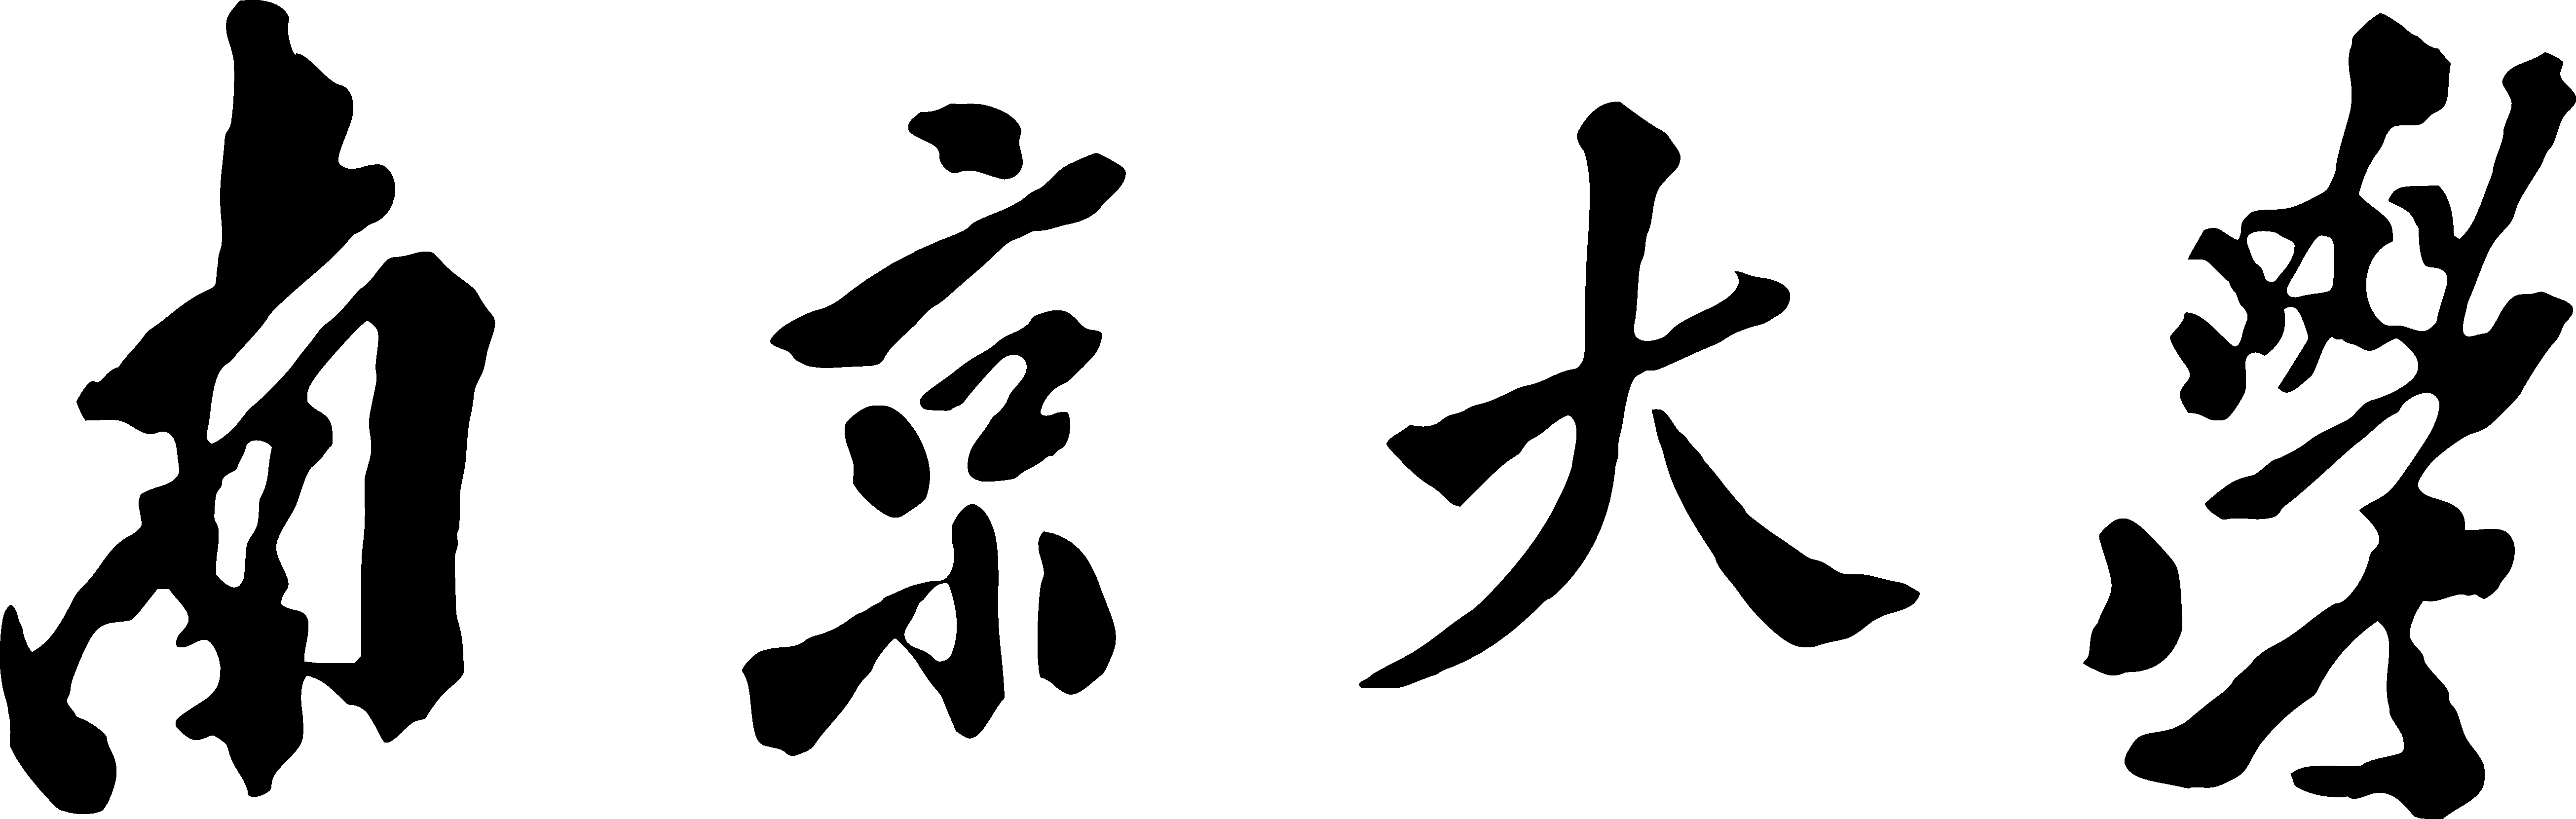
\includegraphics[height=2cm]{name} \\
\vskip 1cm
\zs
\zihao{0} 金~~融~~系~~统~~仿~~真\\
\zihao{1} 学~~期~~报~~告\\
\vskip 2in\zihao{3}
\begin{minipage}{0.9\textwidth}
院\qquad 系\NJUTunderline{\department}\\[3mm]
专\qquad 业\NJUTunderline{\major}\\[3mm]
题\qquad 目\NJUTunderline{\thesistitle}\\[3mm]
年\qquad 级\myuline{4.5cm}{\grade}{\hfill}学\qquad 号\myuline{4cm}{\NJUID}\\[3mm]
学生姓名\NJUTunderline{\myname}\\[3mm]
指导老师\myuline{4.5cm}{\advisor}{\hfill}职\qquad 称\myuline{4cm}{\advisorjob}\\[3mm]
报告提交日期\NJUTunderline{\today}
\end{minipage}
\end{center}
}


\begin{document}
\maketitle
\frontmatter
\normalfont
\begin{abstract}

贷款审批是普通商业银行的一项重大职能环节,在银行风险管理中占据着极其重要的角色。银行通过对借款者的信
用进行评估,便可以更加准确的判断是否批准贷款,以及以多高的利率、多大的款额借给需求方,实现收益管理。
因此,对于银行来说,判断借款者未来是否会违约以及违约大小便成了一个非常重要的问题。\par

本文通过互联网上两组贷款者申请贷款的历史信息记录及其最终违约与否的数据集,结合逻辑回归、分类树和随机森林这
三种方法对借款者未来违约的概率进行预测,并通过准确率,KS统计量,AUC等对三种模型的有效性进行了对比。结果显示随机
森林有效性最高,其次是逻辑回归,最差是分类树。\par

\end{abstract}

\keywords{信用评估;信用风险;逻辑回归;分类树;随机森林}

\pdfbookmark[0]{目录}{tableofcontents}
\tableofcontents
%\listoffigures
%\listoftables  这条命令是表格目录,需要的话可以启用;上面那条是图片目录,不需要可以注释掉或者直接删除

\mainmatter
\zihao{-4}
\song
\chapter{基本介绍}

\section{数据集}

本文通过互联网收集了两组关于借款人申请贷款的相关信息数据集,其基本介绍见表\ref{tab:dataset}。

\begin{table}[htbp]
	\centering
    \caption{\label{tab:dataset}数据集介绍}
    \begin{tabular}{llll}
        \toprule
          数据集来源                      & 数据集名称          & 数据集大小 & 违约比例 \\
        \midrule
		  UCI machine learning repository & German Credit       & 1000       & 30\% \\
		  Kaggle                          & Give me Some Credit & 250,000    & 6.7\% \\
        \bottomrule
    \end{tabular}
\end{table}

\subsection{German Credit}

数据集German Credit的每一条记录包含20个特征变量(代表借款人为了从银行借款所提供的个人信息)以及1个分
类变量(表示最终借款人是否发生了违约)。具体20个特征变量的介绍见表\ref{tab:german}

\begin{table}[htbp]
	\centering
	\caption{\label{tab:german}German Credit数据集特征变量介绍}
	\begin{tabular}{ll}
		\toprule
		   特征变量    & 解释 \\
		\midrule
		   checking    & status of existing checking account\\
		   duration    & duration in month\\
		   history     & credit history \\
		   purpose     & purpose (e.g. car, furniture, repairs, etc.)\\
		   amount      & credit amout \\
		   savings     & savings account/bound \\
		   employ      & present employment since \\
		   installment & installment rate in percentage of disposable income \\
		   status      & personal status and sex \\
		   others      & debtors/guarantors \\
		   residence   & present residence since \\
		   property    & property (e.g. real estate, life insurance, car etc.) \\
		   age         & age in years \\
		   otherplans  & other installment plans \\
		   housing     & housing (e.g. rent, own, for free) \\
		   cards       & number of existing credits at this bank \\
		   job         & job types \\
		   liable      & number of people being liable to provide maintenance for \\
		   tele        & telephone \\
		   foreign     & foreign worker \\
		\bottomrule
	\end{tabular}
\end{table}

\subsection{Give Me Some Credit}
数据集Give me Some Credit的每一条记录包含10个特征变量(代表借款人为了从银行借款所提供的个人信息)以及1个分
类变量(表示最终借款人是否发生了违约)。具体10个特征变量的介绍见表\ref{tab:kaggle}

\begin{table}[htbp]
	\centering
	\caption{\label{tab:kaggle}Give me Some Credit数据集特征变量介绍}
	\begin{tabular}{ll}
		\toprule
		   特征变量                              & 解释 \\
		\midrule
            RevolvingUtilizationOfUnsecuredLines & Total balance on credit cards and personal lines \\
		                                         & of credit except real estate and no installment debt\\
												 & like car loans divided by the sum of credit limits\\
	        Age                                  & Age of borrower in years\\
			NumberOfTime30-69DaysPastDueNotWorse & Number of times borrower has been 30-59 days past\\
			                                     &  due but no worse in the last 2 years\\
			DebtRatio                            & Monthly debt payments, alimony, living costs divided \\
			                                     & by monthly gross income\\
			MonthlyIncome                        & Monthly income \\
			NumberOfOpenCreditLinesAndLoans      & Number of Open loans (installment like car loan \\
			                                     &  or mortgage and) and Lines of credit (e.g. credit cards)\\
		    NumberOfTimes90DaysLate              & Number of times borrower has been 90 days or more \\
			                                     &  past due \\
			NumberRealEstateLoansOrLines         & Number of mortgage and real estate loans including \\
			                                     &  home equity lines of credit \\
			NumberOfTime60-89DaysPastDueNotWorse & Number of times borrower has been 60-89 days past \\
			                                     &  due but no worse in the last 2 years \\
			NumberOfDependents                   & Number of dependents in family excluding themselves \\
			                                     & (spouse, children etc.) \\
		\bottomrule
	\end{tabular}
\end{table}



\chapter{机器学习方法}

首先,我们对原始数据集随机取样其60\%记录作为我们的训练集,其余40\%作为测试集。然后,分别利用逻辑回归、
分类树以及随机森林对于训练集进行监督式学习,得到相应的分类器。

\section{逻辑回归}
\subsection{逻辑回归简介}

传统的线性回归$y = \theta x$(其中$\theta$为特征变量的系数行向量,$x$为特征变量列向量)所得到的因变量$y$
的取值范围往往在整个实数空间内,而一般的分类问题只有可数个因变量取值。逻辑回归利用逻辑函数$h(z) = \frac{1}{1+e^{-z}}$(其中$z=\theta x$)将实数空间内的数映射到[0, 1]上,使得连续问题转化为离散问题的``概率''解(见图\ref{fig:logistic})。

\begin{figure}
\centering
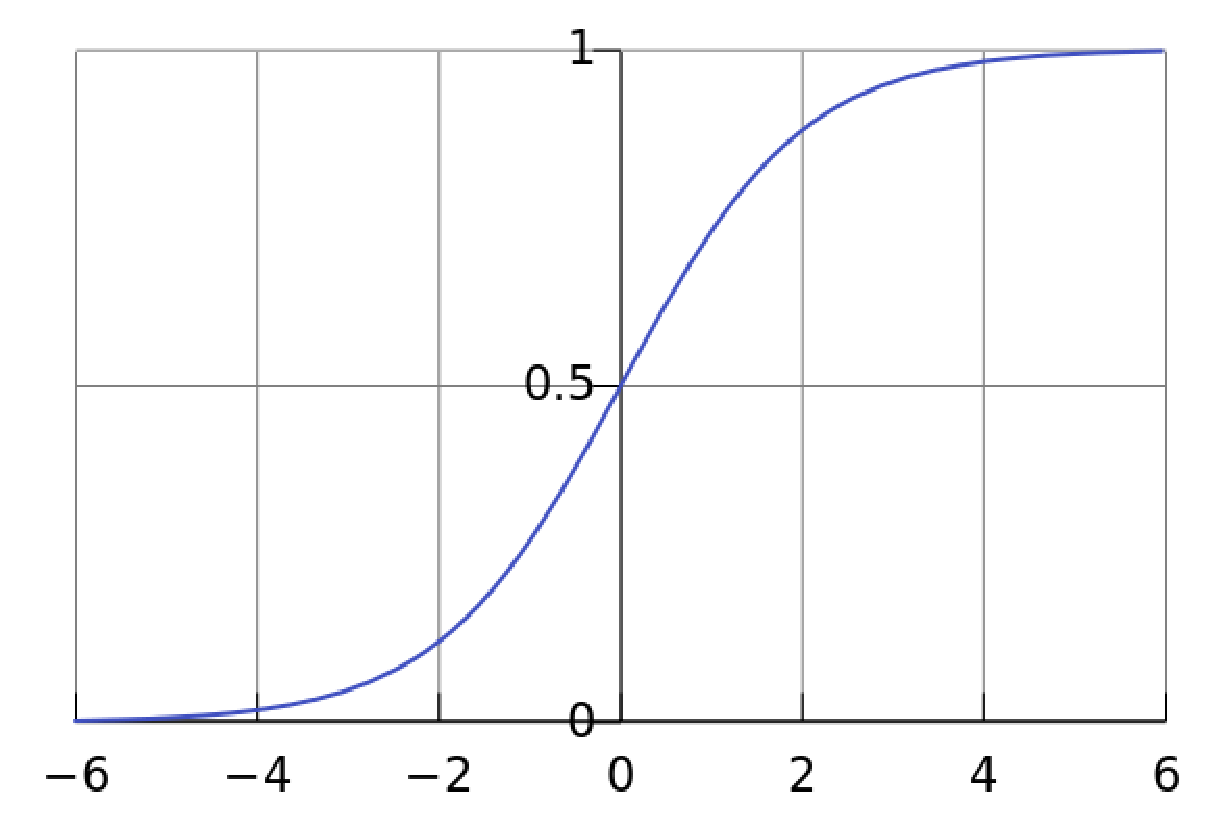
\includegraphics[width=0.8\linewidth]{logit.pdf}
\caption{\label{fig:logistic}逻辑函数}
\end{figure}

\subsection{逻辑回归算法}
其合理性是由于在分界线(面,见图\ref{fig:bound})上的数据点的$z$值为0,通过逻辑函数映射到0.5,代表分解线(面)上的数据点
无法判断其类别,可以理解为有50\%的概率为Negative Class,有50\%的概率为Positive Class;分界线(面)把多维空间
分为了两个部分,其中正向空间内离分界线(面)越远$z$值越大,通过逻辑函数映射到1,代表正向空间内远离分界线(面)
的数据点有很大的可能性为Positive Class。

\begin{figure}
\centering
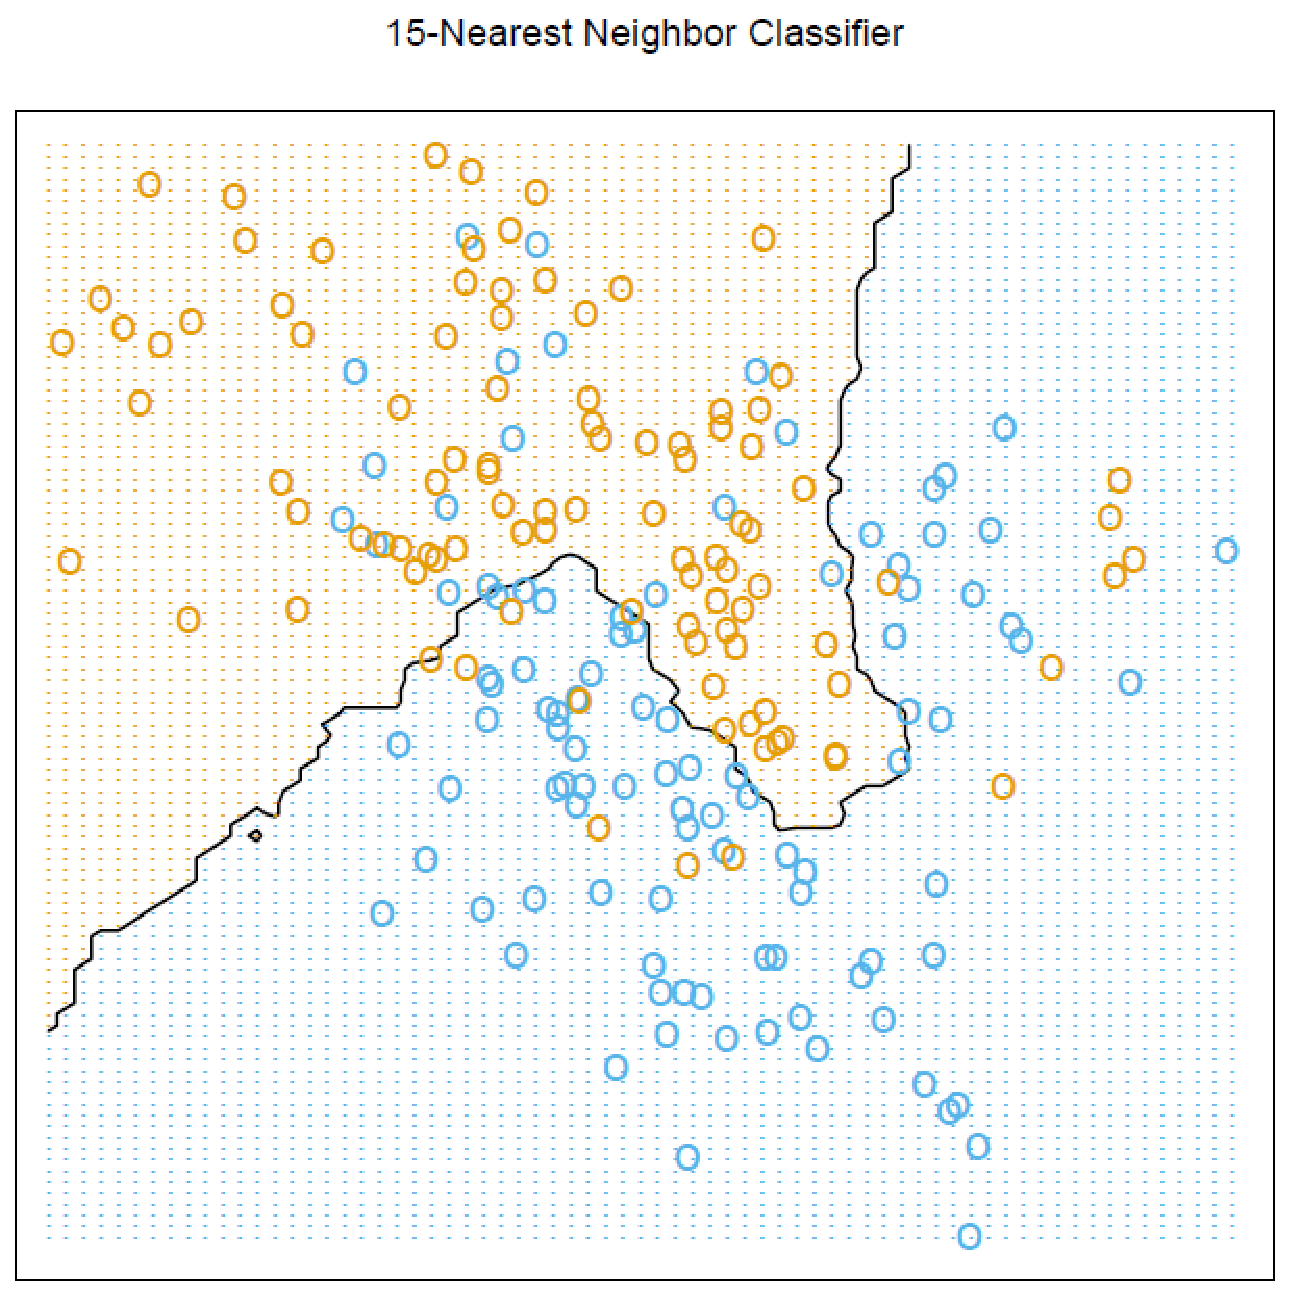
\includegraphics[width=0.8\linewidth]{bound.pdf}
\caption{\label{fig:bound}分界线}
\end{figure}

具体的特征向量系数$\theta$通过最小化成本函数$cost(\theta) = y log(h(\theta x)) + (1-y) log(1-h(\theta x))$
便可获得,这样就得到了逻辑回归分类器。

\subsection{逻辑回归结果}
这里以German Credit的数据为例,表\ref{tab:logit}显示了逻辑回归特征变量系数及其显著性。

\begin{table}[htbp]
  \centering
    \caption{\label{tab:logit}逻辑回归结果}
    \begin{tabular}{lllll}
    \toprule
          & Estimate & Std. Error & z value & $Pr(\ge\|z\|)$ \\
    \midrule
    (Intercept) & -5.48743 & 1.387014 & -3.95629 & 7.61E-05 ***\\
    checking & 0.484832 & 0.089609 & 5.41055 & 6.28E-08 ***\\
    duration & -0.01426 & 0.01144 & -1.24679 & 0.212473 \\
    history & 0.469549 & 0.114837 & 4.088823 & 4.34E-05 ***\\
    purpose & 0.068907 & 0.042475 & 1.622316 & 0.104736 \\
    amount & -0.00015 & 5.07E-05 & -2.99869 & 0.002711 ***\\
    savings & 0.25071 & 0.076253 & 3.287871 & 0.001009 ***\\
    employed & 0.109647 & 0.095728 & 1.145409 & 0.25204 \\
    installp & -0.33189 & 0.106943 & -3.10348 & 0.001913 ***\\
    marital & 0.48904 & 0.155785 & 3.139197 & 0.001694 ***\\
    coapp & 0.100784 & 0.225263 & 0.447406 & 0.654582 \\
    resident & -0.10415 & 0.101927 & -1.02184 & 0.306856 \\
    property & -0.14986 & 0.12051 & -1.24353 & 0.213674 \\
    age   & 0.019083 & 0.011009 & 1.73332 & 0.083039 *\\
    other & 0.325128 & 0.140454 & 2.314837 & 0.020622 **\\
    housing & 0.274481 & 0.216319 & 1.268869 & 0.204488 \\
    existcr & -0.39916 & 0.203087 & -1.96544 & 0.049364 **\\
    job   & 0.34085 & 0.179191 & 1.902159 & 0.057150 *\\
    depends & -0.24825 & 0.290759 & -0.8538 & 0.393214 \\
    telephon & 0.021655 & 0.244287 & 0.088645 & 0.929364 \\
    foreign & 1.699978 & 0.891746 & 1.906348 & 0.056605 *\\
    \bottomrule
    \end{tabular}%
  \label{tab:logit}%
\end{table}%

除此之外,对于拒绝给予贷款的申请人我们给出了三项最有可能导致被拒的原因,见图\ref{fig:topk}

\begin{figure}
\centering
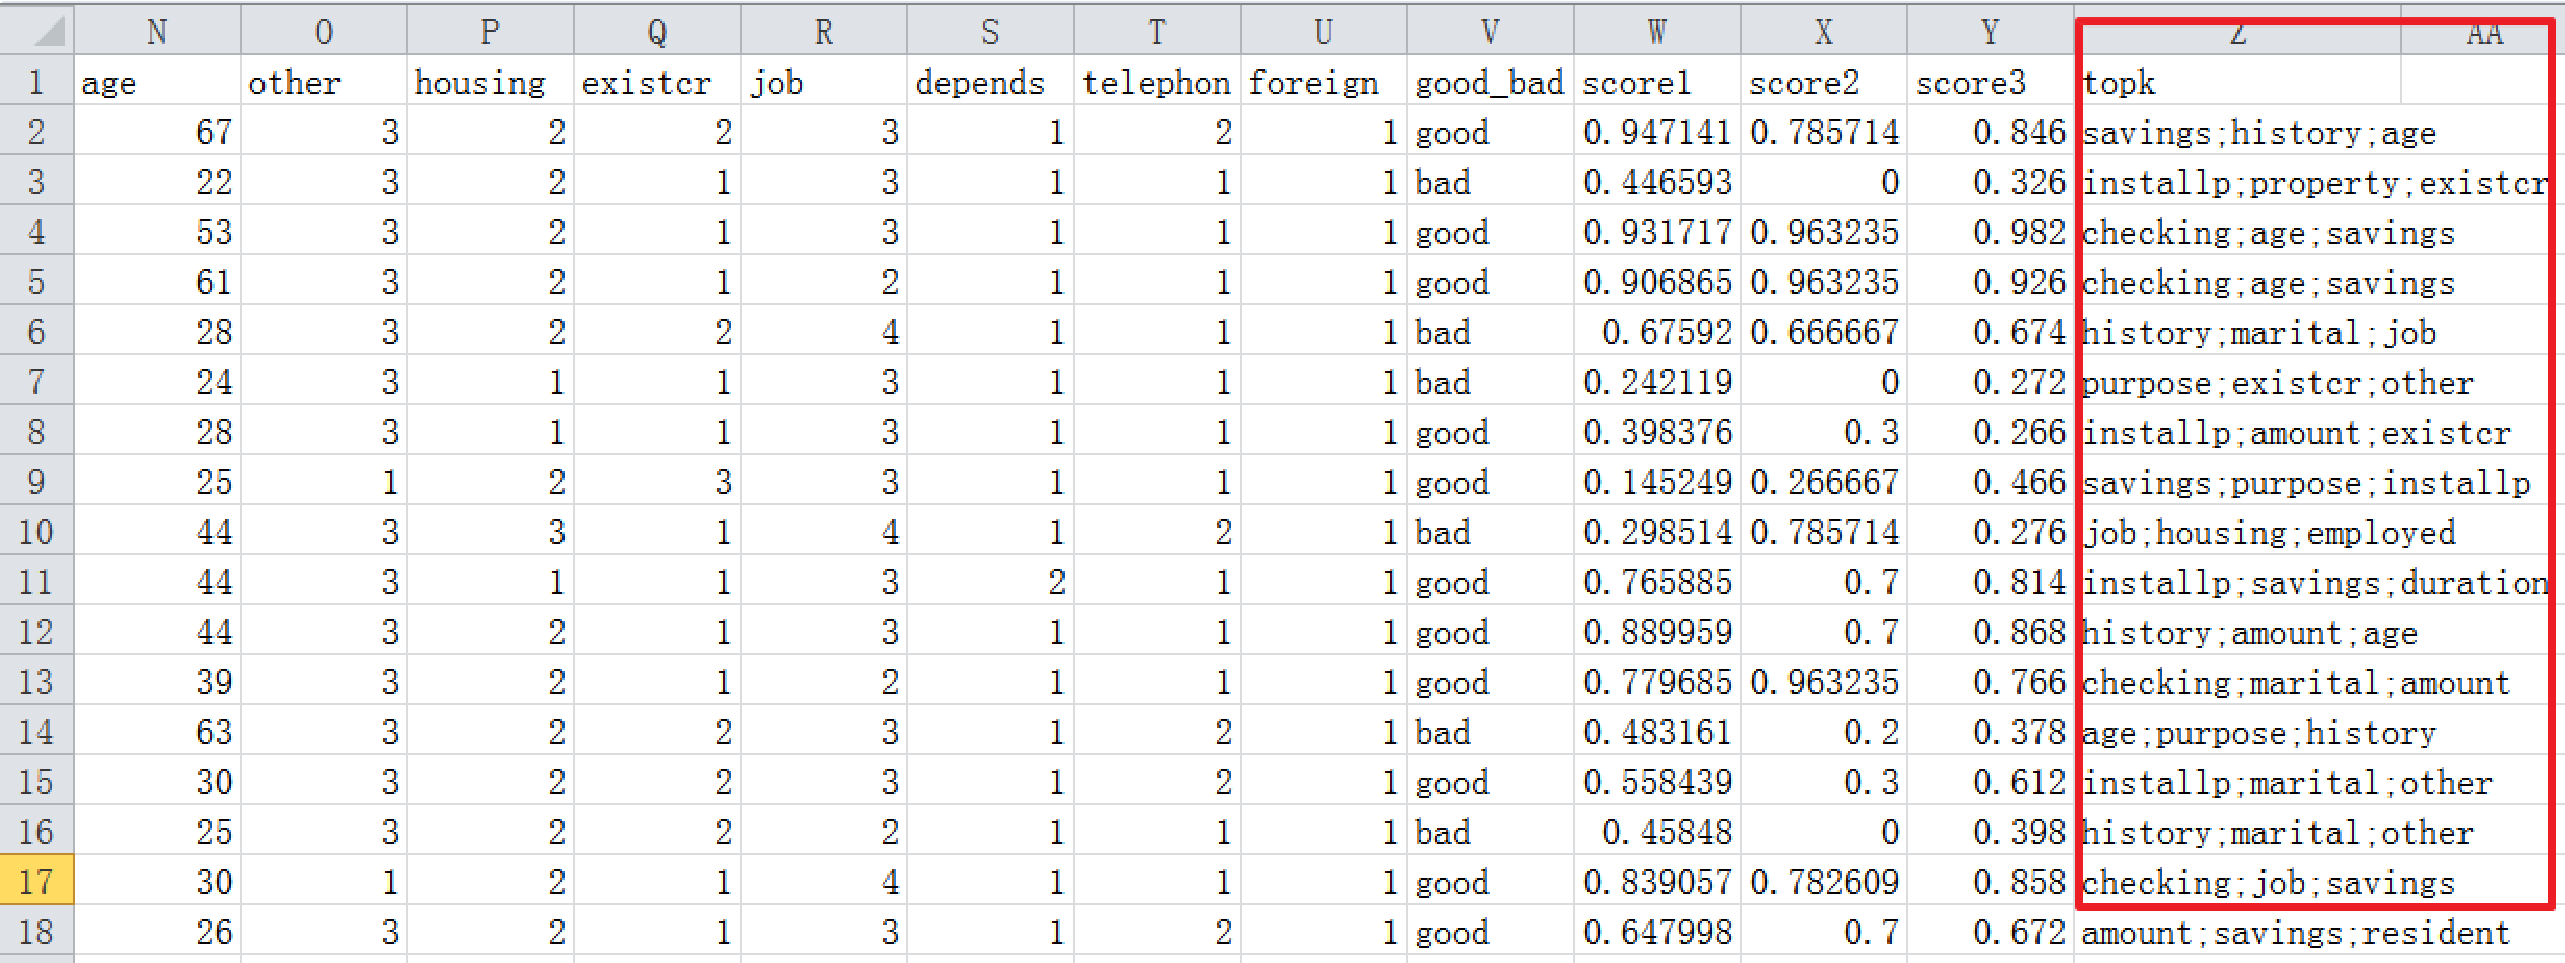
\includegraphics[width=0.8\textwidth]{topk.pdf}
\caption{\label{fig:topk}导致贷款被拒最有可能的三项原因}
\end{figure}

\section{分类树}
\subsection{分类树简介}
分类树通过对数据集按照不同的标准进行分枝,直至无法再分为止。其叶结点表示最终分类结果,其余节点表示各个
分类逻辑表达式。分类树建立的难点在于如何选取分类标准以及相应阈值。传统的ID3是使用信息熵来刻画数据集
的纯度,并选择使得信息增益最大的分类标准作为非叶结点的分裂标准。

\subsection{分类树算法}
数据集$S$的纯度可以用其信息熵来刻画:$H(S) = - \sum _{i} p(i) log(p(i))$,其中$p(i)$表示种类$i$出现的
频率,可见若数据集$S$中的数据只有一类的话,信息熵达到最小值0。其次,非叶节点的分裂标准通过选择使得信息
增益$IG(Y) = H(S) - \sum_{i \in T} p(i) log(p(i))$最大的分类标准(式中子数据集$T$表示按此分类标准
得到的子数据集)。

\subsection{分类树结果}
分类树的结果如图\ref{fig:classification},因为图像显示问题,这里的根节点应为$checking \le 2.5$。
\begin{figure}
\centering
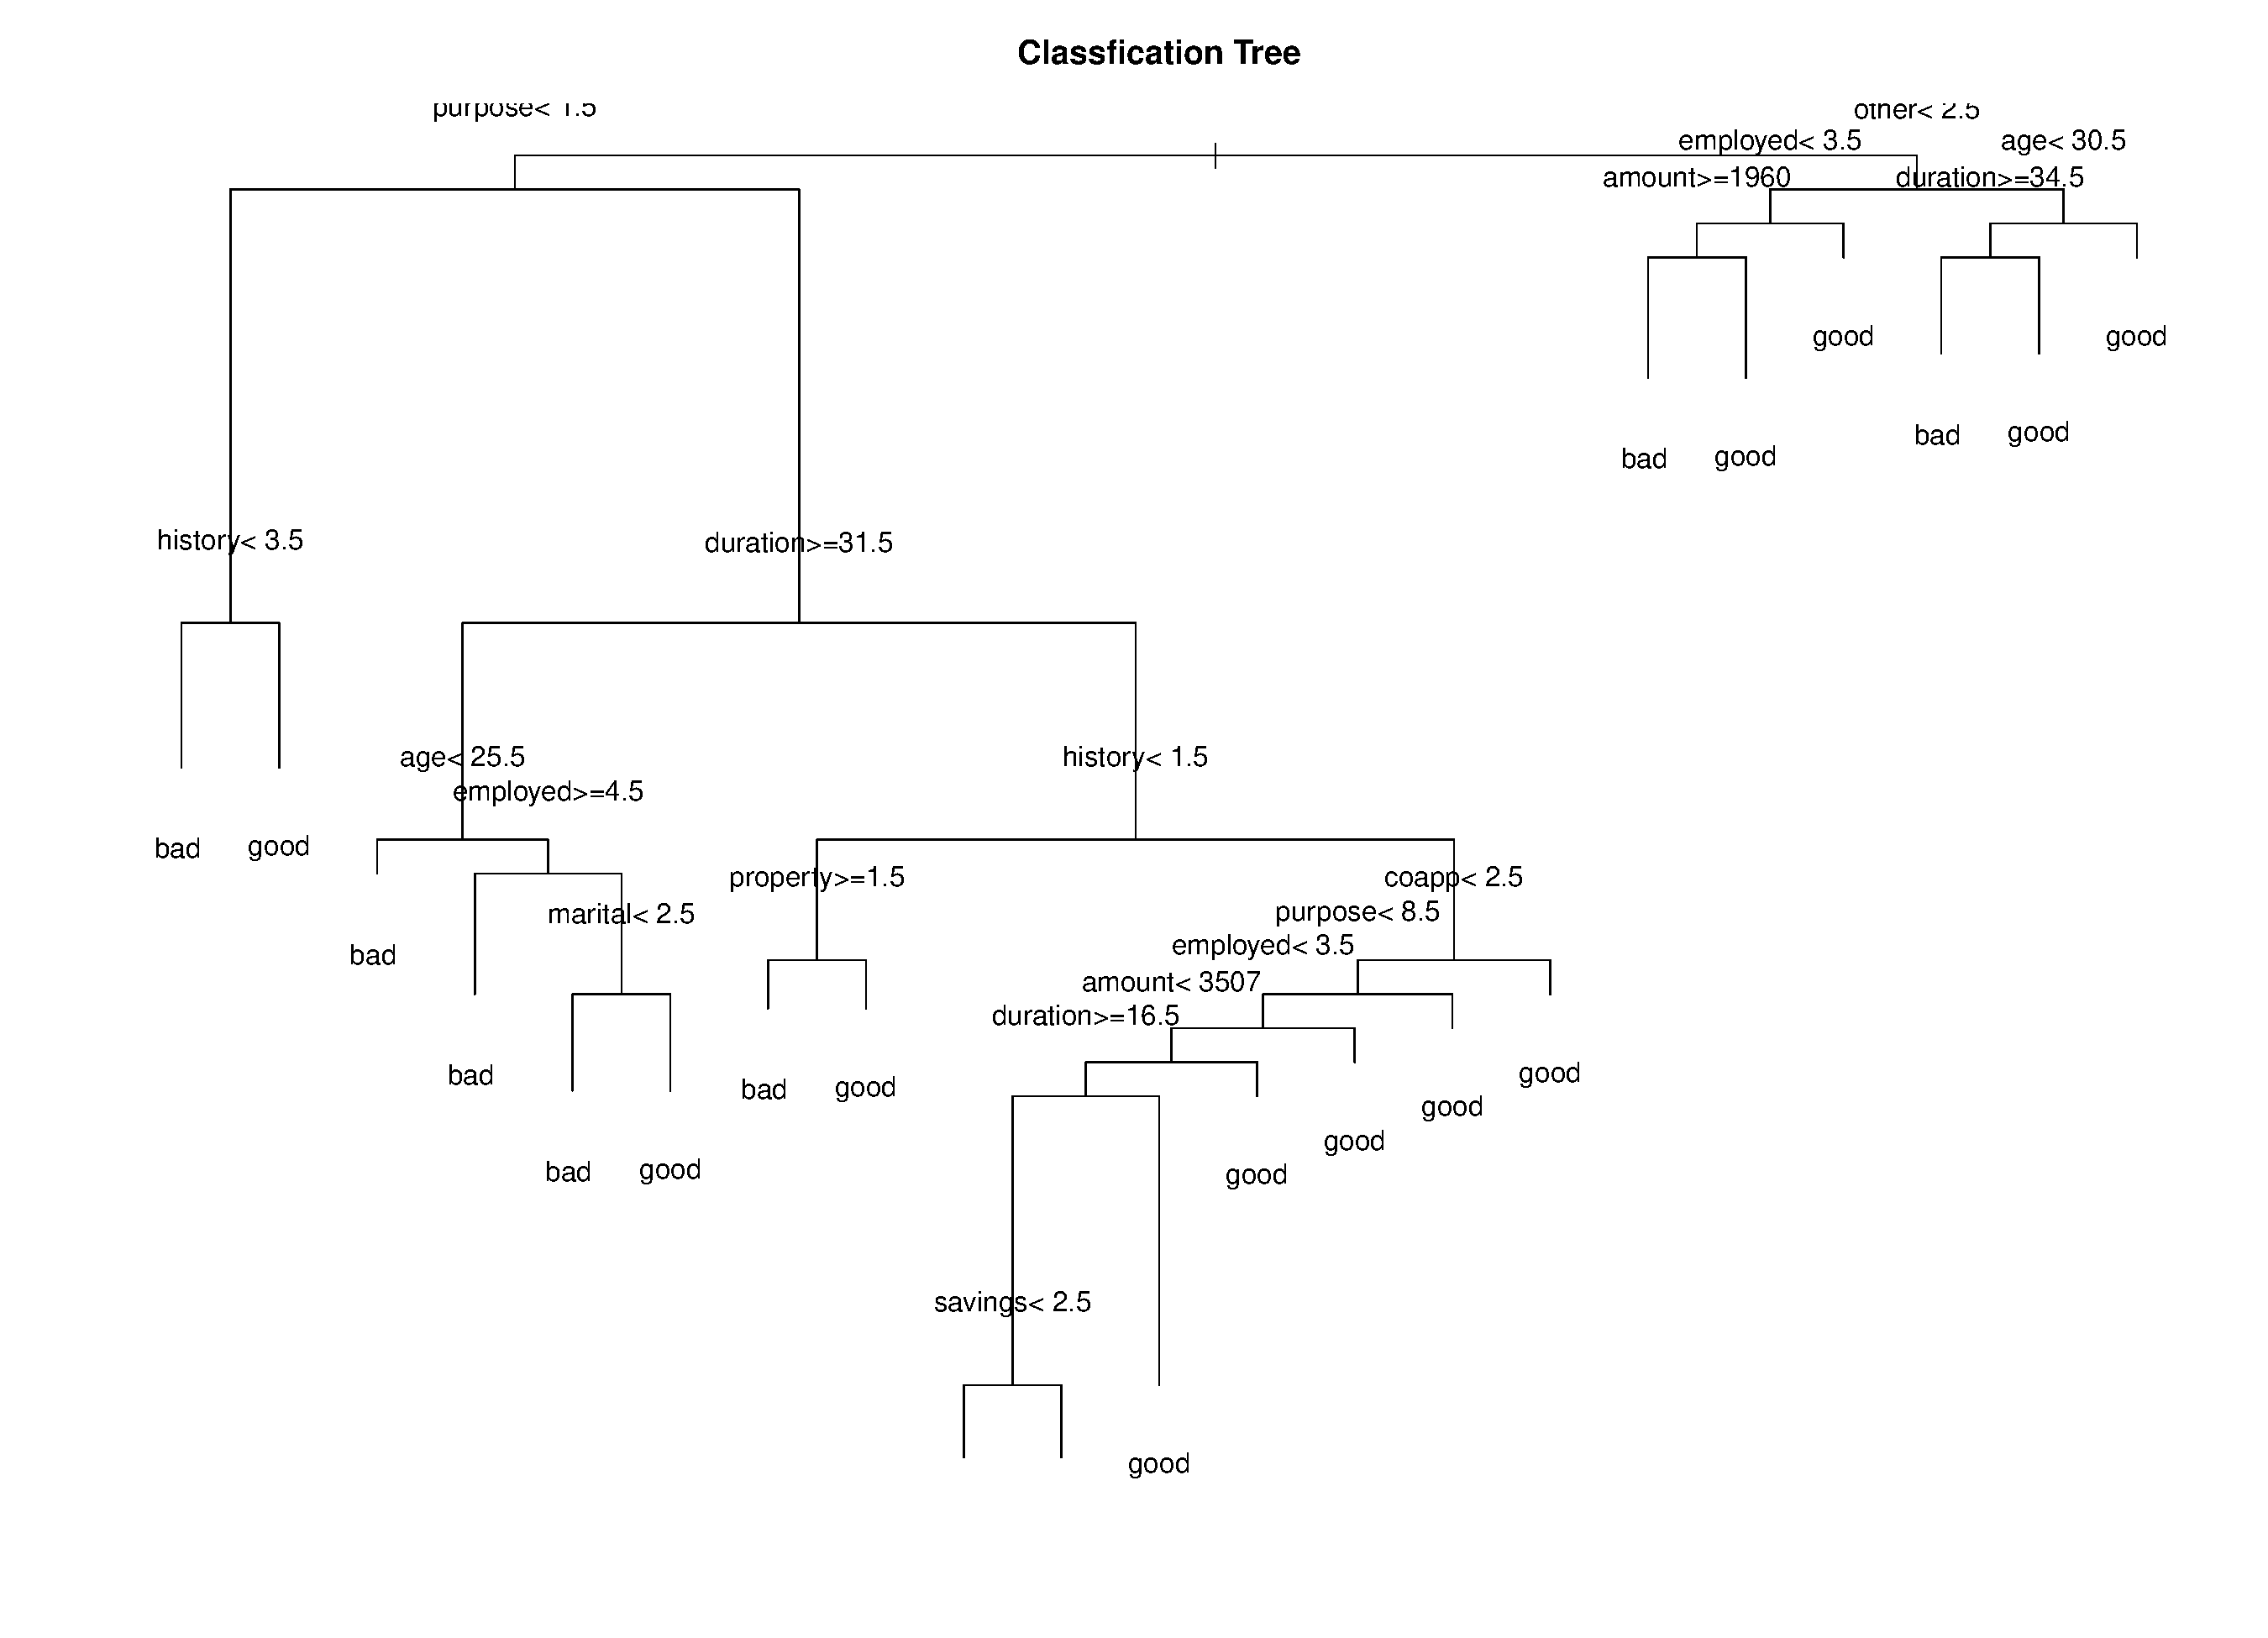
\includegraphics[width=0.8\textwidth]{classificationtree.pdf}
\caption{\label{fig:classification}分类树结果}
\end{figure}

\section{随机森林}

\subsection{随机森林简介}
随机森林是一种集成式学习方法,包含了多个分类树分类器,最终的分类结果由众多分类器投票得出。随机森林因为其
计算效率高、适用于并行处理、可以处理大量数据、评估变量重要性,在最近几年机器学习领域比较流行。微软的体感
游戏设备Kinect也利用了随机森林来识别玩家的动作。

\subsection{随机森林算法}
随机森林是以分类树为基础的集成式学习方法,与其相比,主要有两大区别:
\begin{itemize}
	\item 每棵分类树所使用的数据集是通过自助法对原始数据集进行有放回重取样得到的。
	\item 每棵分类树训练所用的特征变量是随机给定的。
\end{itemize}
最终的分类结果由各棵分类树投票得出。

\subsection{随机森林结果}
随机森林得到的特征变量重要性如图\ref{fig:varimp}
\begin{figure}
\centering
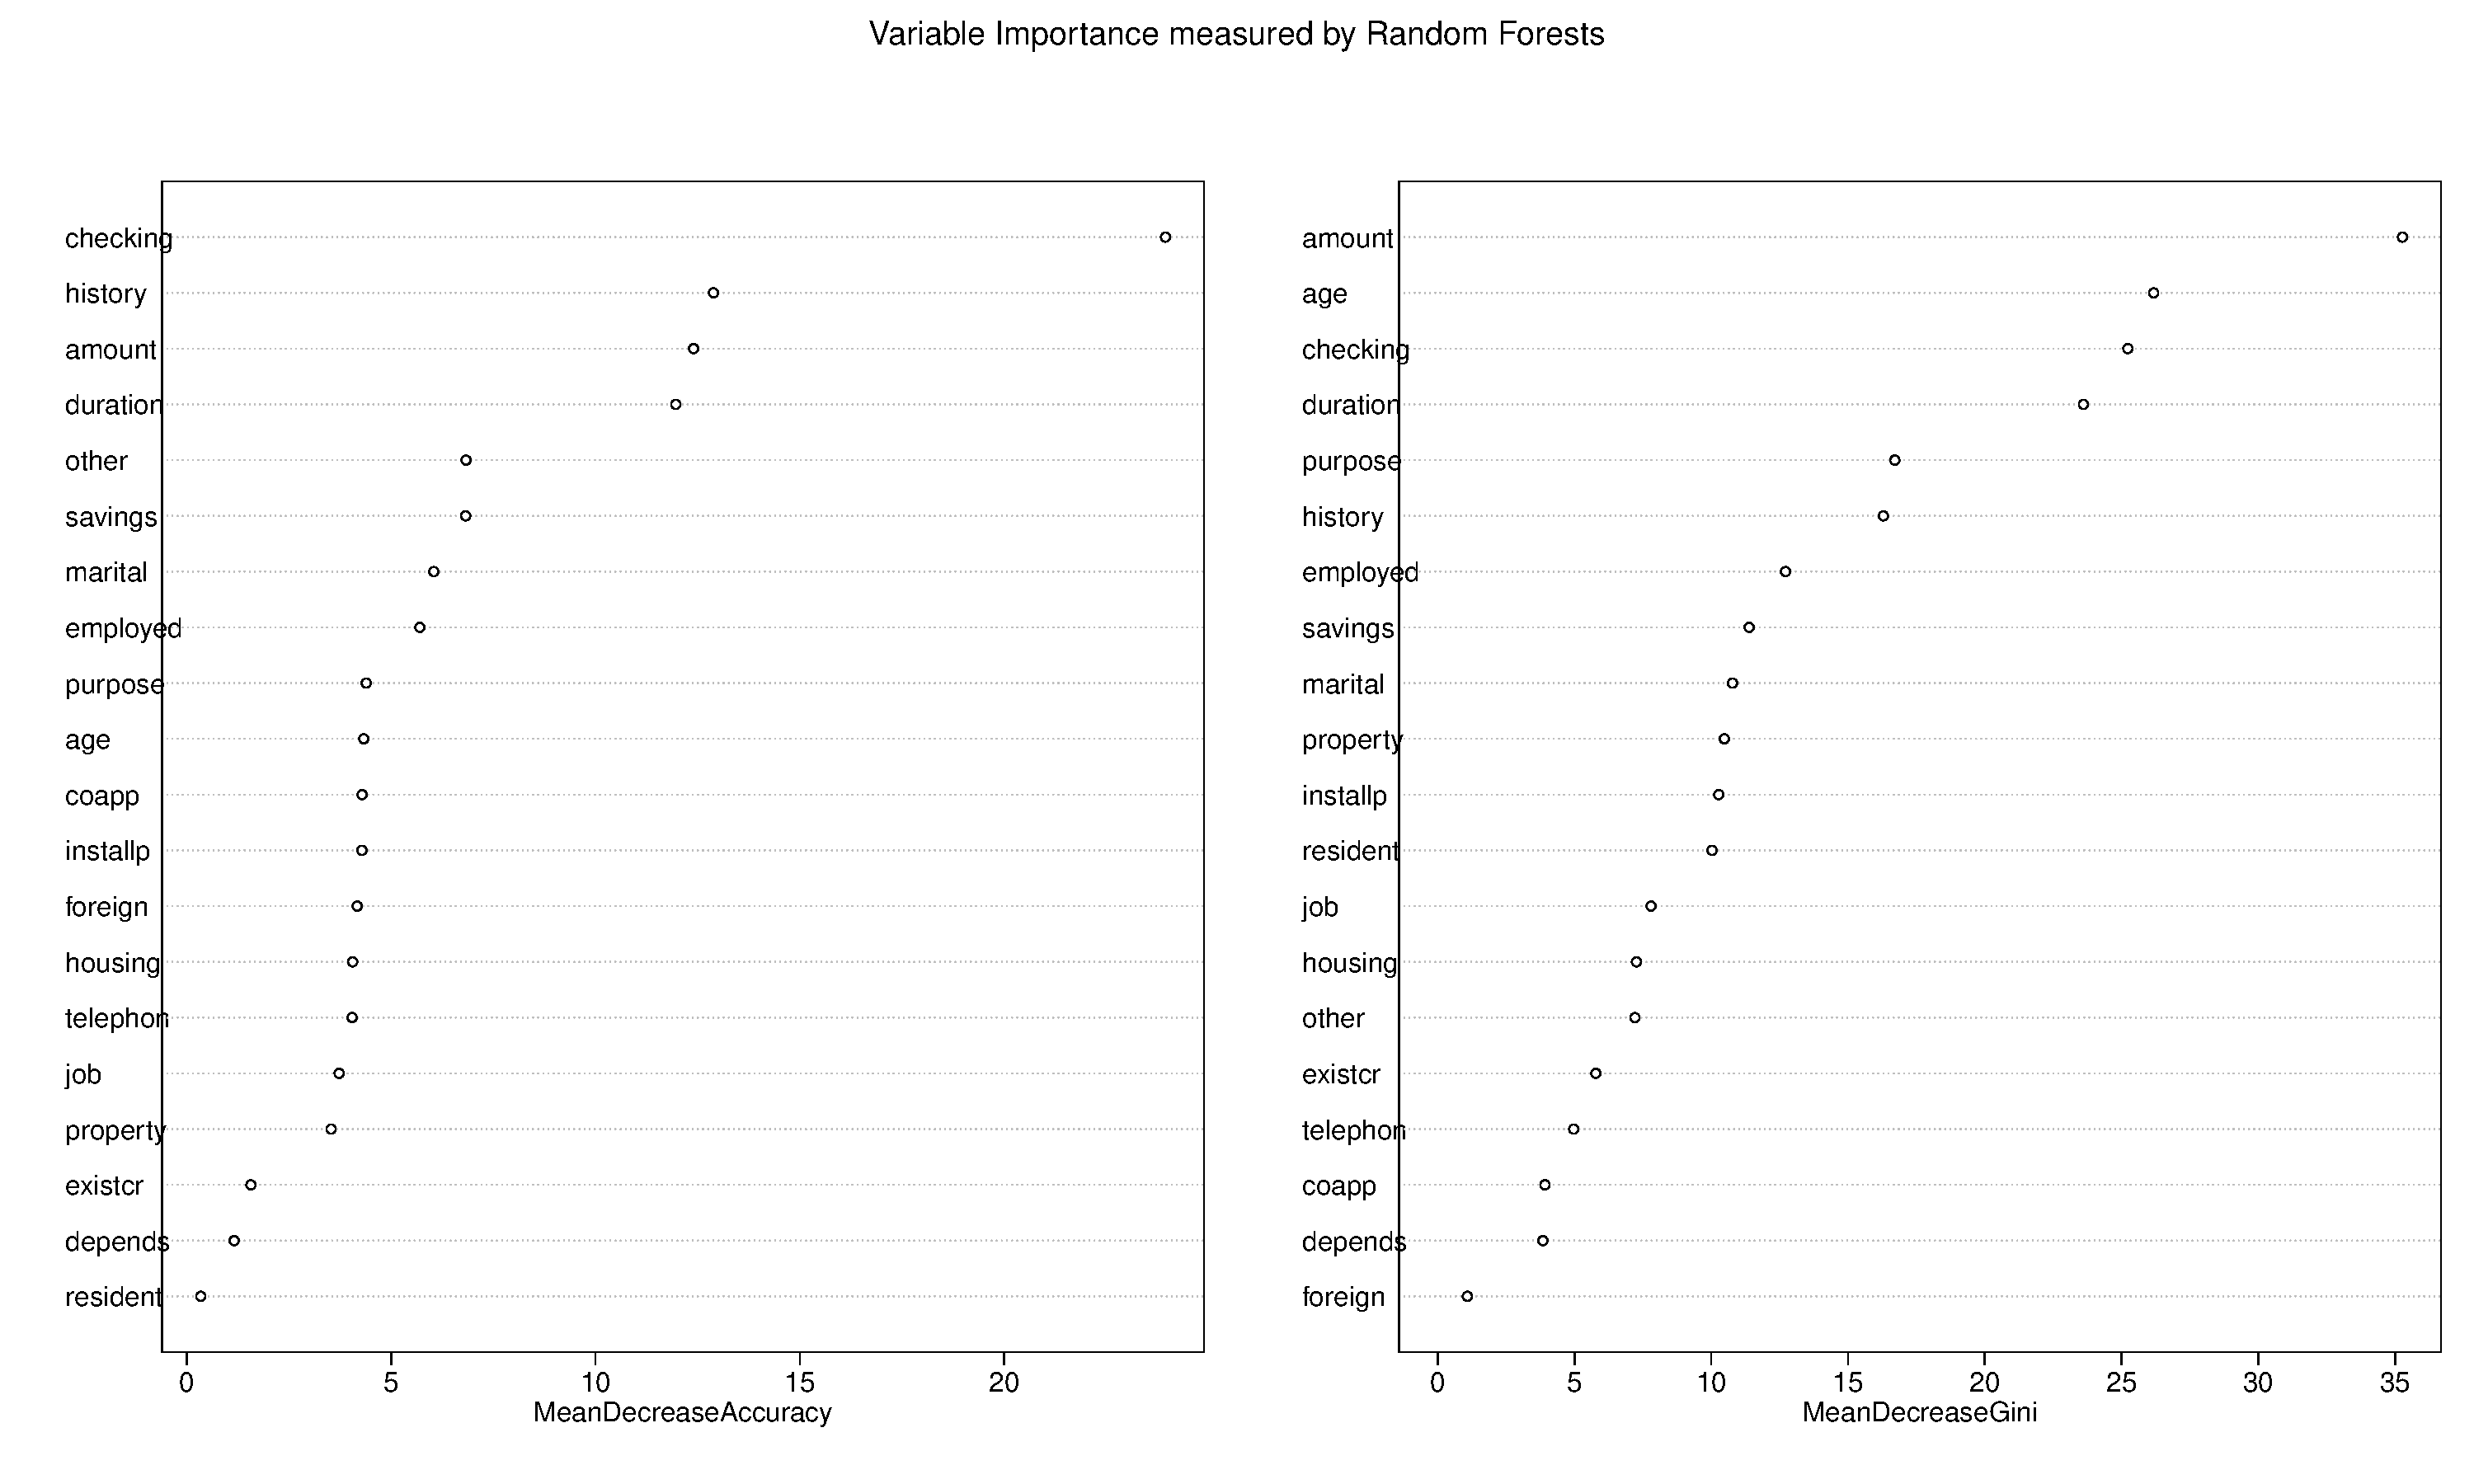
\includegraphics[width=0.8\linewidth]{varimp.pdf}
\caption{\label{fig:varimp}特征变量重要性}
\end{figure}







\chapter{模型评估}

\section{模型评估标准}
我们选取了准确率,KS统计量以及AUC作为三种模型的评估标准,为了理解这三种评估标准,首先介绍一下分类问题
的最终可能几种结果,见表\ref{tab:roc}。

\begin{table}[htbp]
  \centering
    \begin{tabular}{rrr}
    \toprule
          & \multicolumn{2}{c}{真实值} \\
    \midrule
    \multicolumn{1}{c}{\multirow{2}[0]{*}{预测值}} & 真阳(TP) & 伪阳(FP) \\
    \multicolumn{1}{c}{} & 伪阴(FN) & 真阴(TN) \\
    \bottomrule
    \end{tabular}%
  \label{tab:roc}%
\end{table}%

其中准确率等于$\frac{TP+TN}{TP+FP+FN+TN}$,KS统计量以及AUC是通过接受者操作特征曲线(ROC曲线)得到的。
ROC曲线的横坐标为$False Positive Rate = \frac{FP}{FP+TN}$,纵坐标为$TRUE Positive Rate = \frac{TP}{TP+FN}$
(见如\ref{fig:roc})。其中KS统计量为纵坐标与横坐标差值的最大值,AUC为ROC曲线与横坐标所围的面积,其理想值
为1。

\begin{figure}
\centering
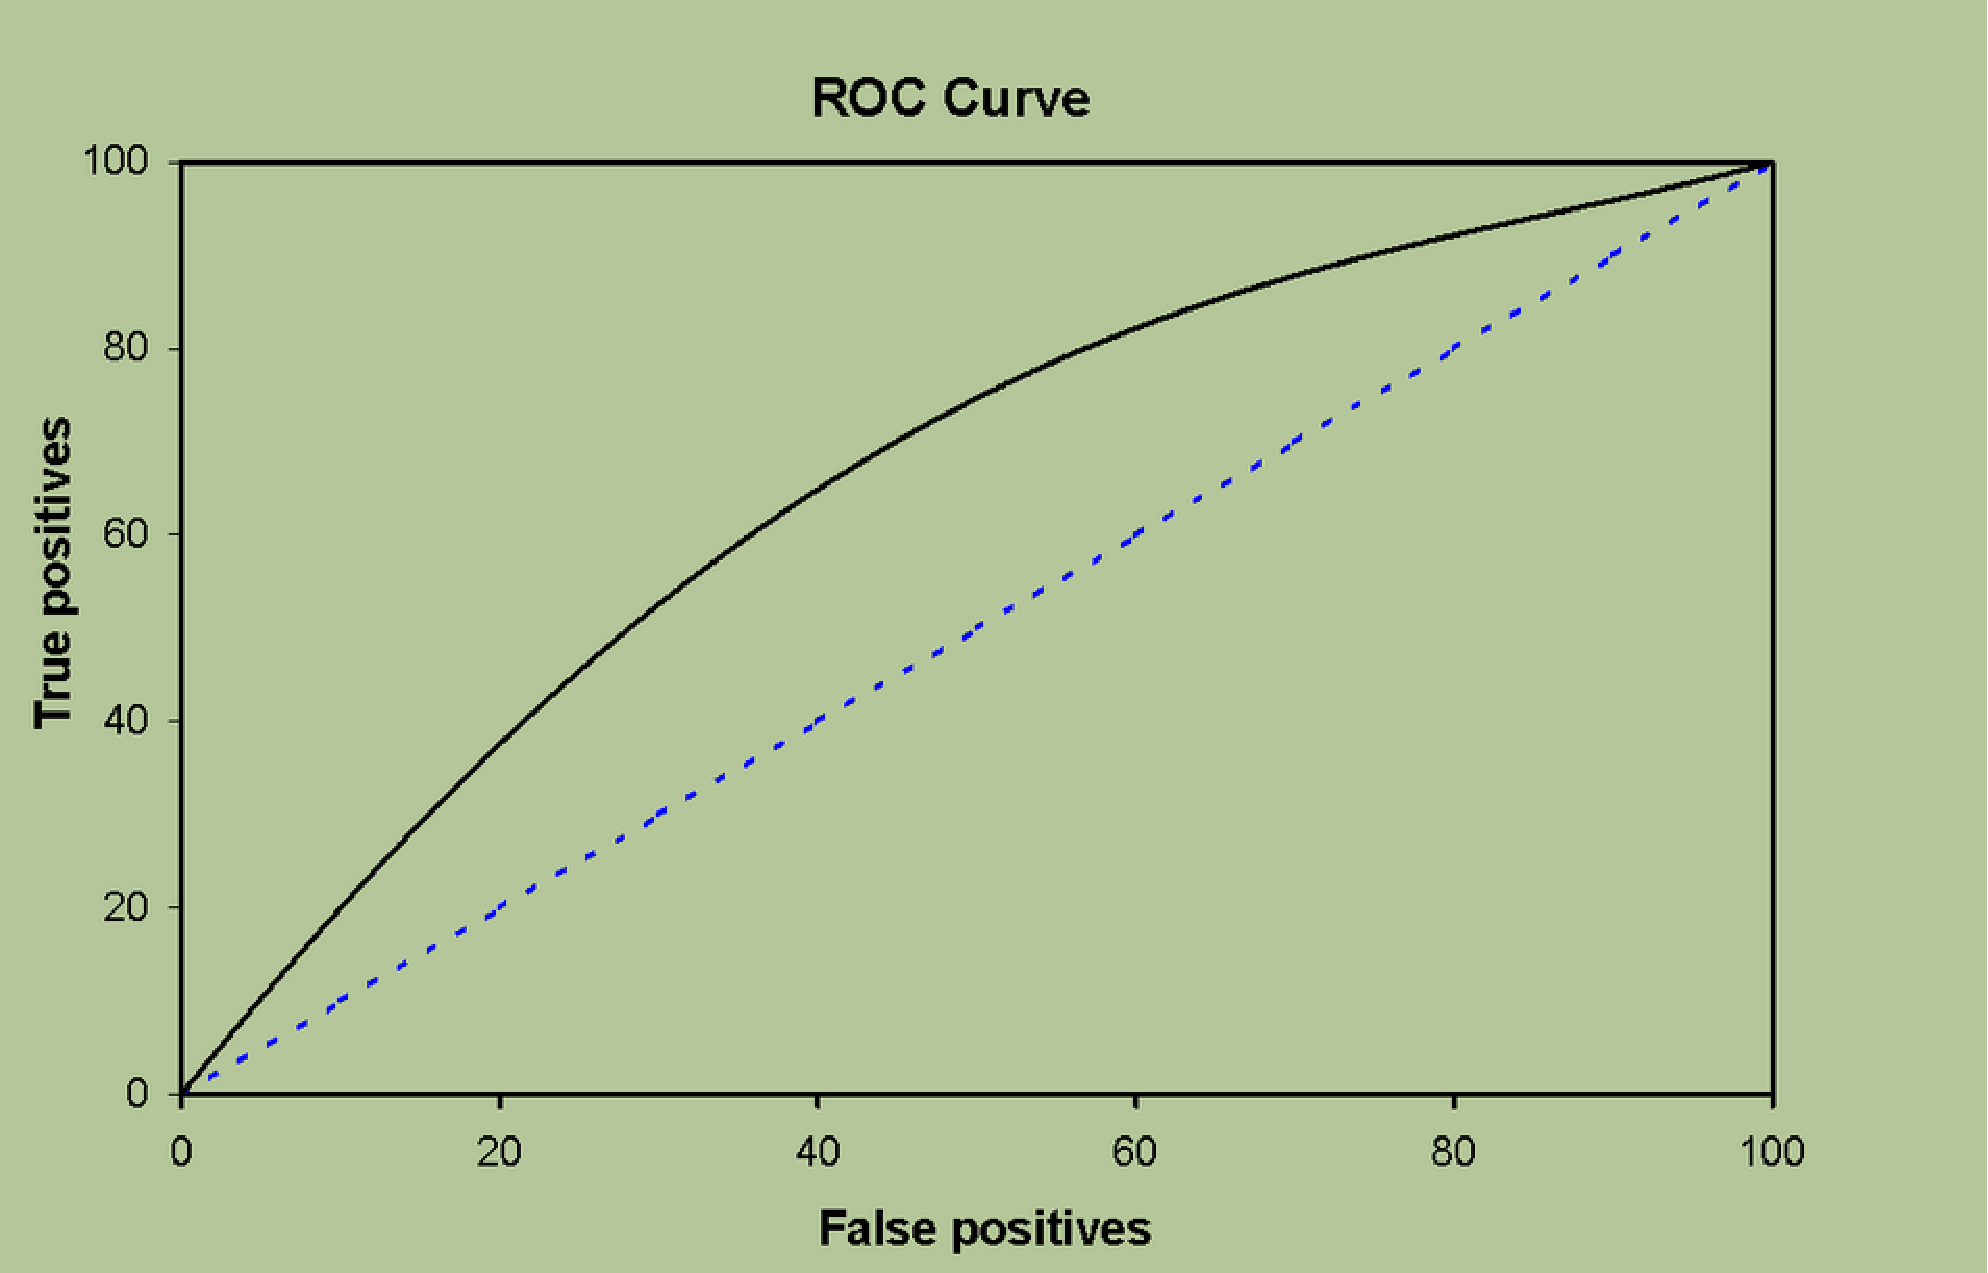
\includegraphics[width=0.8\linewidth]{roc.pdf}
\caption{\label{fig:roc}接受者操作特征曲线(ROC)}
\end{figure}

\section{模型评估结果}
\subsection{German Credit}
以German Credit为训练数据,得到以下结果:

\begin{figure}
\centering
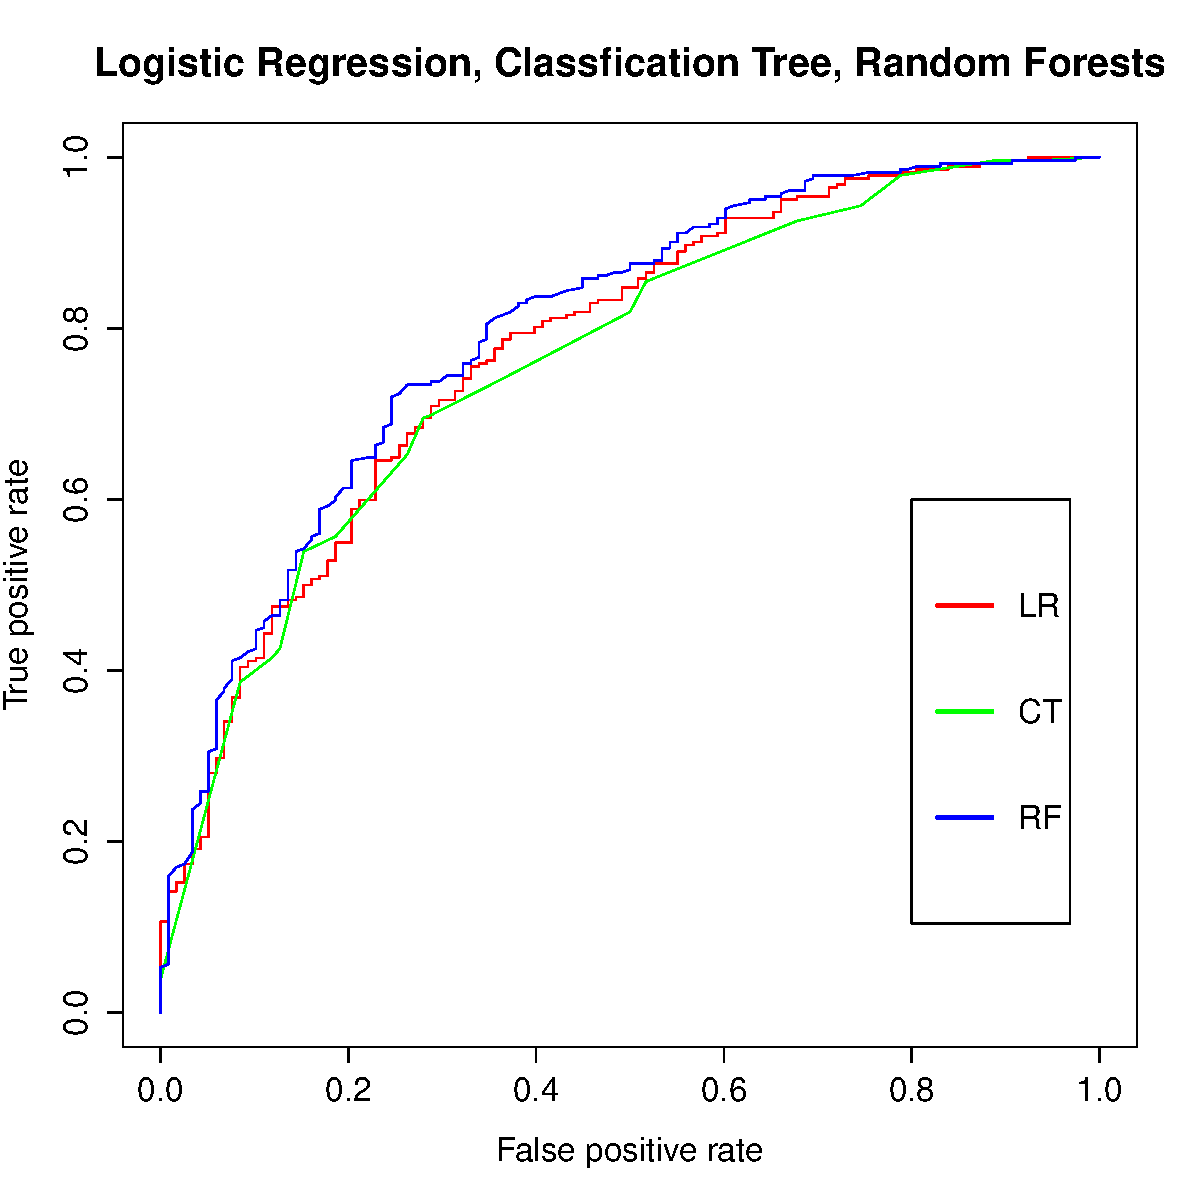
\includegraphics[width=0.8\linewidth]{roc1.pdf}
\caption{\label{fig:roc1}German Credit - ROC}
\end{figure}

\begin{table}[htbp]
  \centering
  \caption{German Credit}
    \begin{tabular}{lllll}
    \toprule
    Model & KS  & AUC & Accuracy  & Cutoff \\
    \midrule
    LR & 0.425 & 0.776 & 0.773 & 0.421 \\
    CT & 0.415 & 0.762 & 0.753 & 0.250 \\
    RF & 0.474 & 0.798 & 0.780  & 0.472 \\
    \bottomrule
    \end{tabular}%
  \label{tab:roc1}%
\end{table}%

\subsection{Give Me Some Credit}
以Give Me Some Credit为训练数据,得到以下结果:
\begin{figure}
\centering
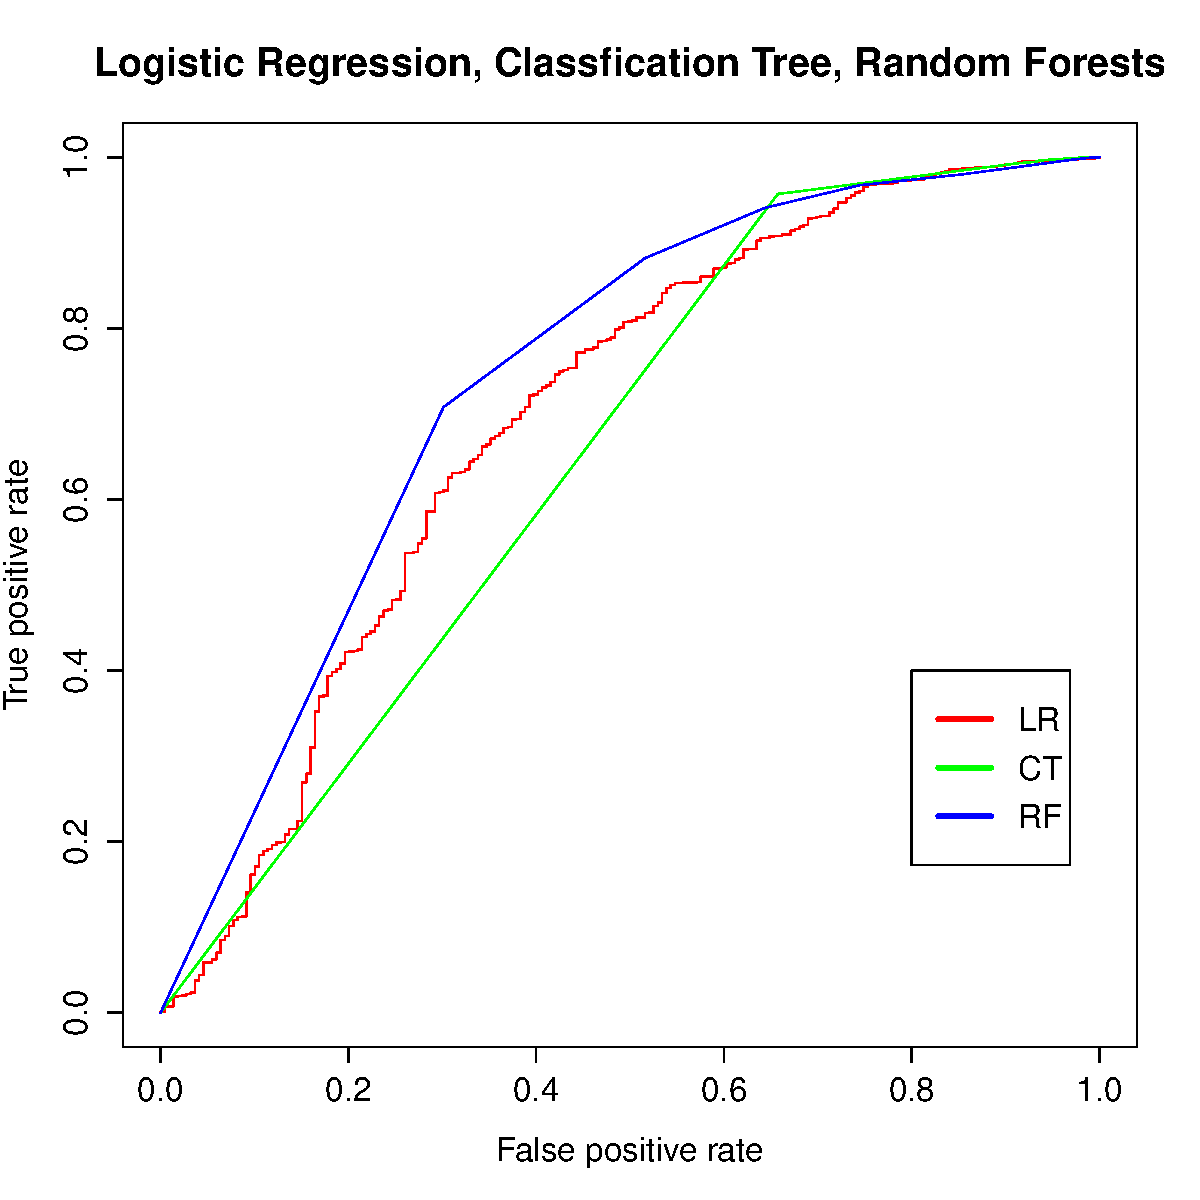
\includegraphics[width=0.8\linewidth]{roc2.pdf}
\caption{\label{fig:roc2}Give Me Some Credit - ROC}
\end{figure}

\begin{table}[htbp]
  \centering
  \caption{Give Me Some Credit}
    \begin{tabular}{lllll}
    \toprule
    Model & KS  & AUC & Accuracy  & Cutoff \\
    \midrule
    LR & 0.329 & 0.695 & 0.933 & 0.727 \\
    CT & 0.300 & 0.651 & 0.933 & 0.308 \\
    RF & 0.407 & 0.741 & 0.932 & 0.300 \\
    \bottomrule
    \end{tabular}%
  \label{tab:roc2}%
\end{table}%

\chapter{结论}
通过以上模型评估结果我们可得到如下结果:
\begin{itemize}
	\item 随机森林的效果最佳,其次是逻辑回归,分类树表现最差。
	\item 随机森林与分类树的对比可以看出集成式学习的优势。
	\item 随机森林可以通过和逻辑回归结合起来以提高其效果。
\end{itemize}

%\backmatter
%\pagenumbering{Roman}
% 参考文献
%\bibliographystyle{unsrt}
%\bibliography{ref/reference}
%\addcontentsline{toc}{chapter}{参考文献}

\end{document}